


\section{Goals of Crypto}

\subsubsection{Confidentality}

\subsubsection{Integrity}
we make sure that the received message is equal to the sent one


\subsubsection{Authenticated}
we make sure about who sent the message

\section{Some Historic Examples}

\subsection{Substitution Cipher: Caesar Cipher}


\subsubsection{How to break a substitution cipher}

\begin{enumerate}
    \item use frequency of English letters
    \item use frequency of pairs of letters
\end{enumerate}


\subsection{Vigener Cipher}

The format of Vigener Cipher is shown in Figure \ref{fig: 01 Vigener Cipher}.

\begin{figure}
    \centering
    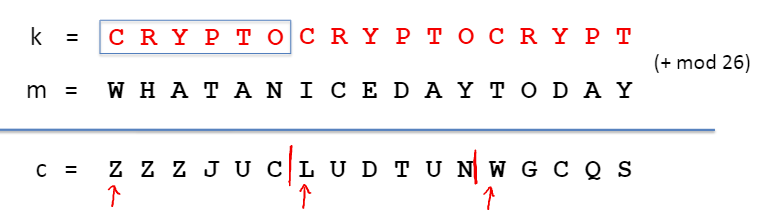
\includegraphics[width=0.8\textwidth]{Stanford_Crypto_1/fig/01_Introduction/Vigener Cipher.png}
    \caption{Vigener Cipher}
    \label{fig: 01 Vigener Cipher}
\end{figure}


\section{Introduction of Discrete Probability}


\subsection{Randomized Algorithms}

\subsubsection{Deterministic Algorithm}

$$y \leftarrow A(m)$$. 

\subsubsection{Randomized Algorithm}

$$
y \longleftarrow A(m ; r) \quad \text { where } \quad r \longleftarrow\{0,1\}^{n}
$$

So the output of $A(m)$ is a random variable

$$
\mathrm{y} \leftrightarrow \mathrm{A}(\mathrm{m})
$$



\subsection{An Important Property of XOR}

\begin{theorem} [An Important Property of XOR]  An Important Property of XOR:
    $Y$ a \textbf{rand. var.} over $\{0,1\}^{n}, \quad X$ an \textbf{indep. uniform var.} on $\{0,1\}^{n}$
    Then $Z:=Y \oplus X$ is uniform var. on $\{0,1\}^{n}$
    
\end{theorem}


\subsection{The Birthday Paradox}

\begin{theorem} [The Birthday Paradox] The Birthday Paradox:

    Let $r_{1}, \ldots, r_{n} \in U \quad$ be indep. identically distributed random vars.
    when $\mathrm{n}=1.2 \times|\mathrm{U}|^{1 / 2}$ then $\operatorname{Pr}\left[\exists \mathrm{i} \neq \mathrm{j}: r_{\mathrm{i}}=r_{\mathrm{j}}\right] \geq 1 / 2$
    
\end{theorem}

\section{Semantic Security}

Here, we summarized different Semantic Security Models and Definitions.